% Document settings
\documentclass[a4paper,11pt]{article}

% Packages
  % math formulas
\usepackage{amsmath,amsthm,amssymb}
  % graphics
\usepackage{graphicx}
\usepackage{wrapfig}
  % plots
\usepackage{pgfplots}
  % other
\usepackage[warn]{mathtext}
\usepackage{cmap}
\usepackage[T1,T2A]{fontenc}
\usepackage[utf8]{inputenc}
\usepackage[english,russian]{babel}

% Package settings
%% graphicx
\graphicspath{{Pictures/}}
\DeclareGraphicsExtensions{.pdf,.png,.jpg}
%% pgfplots
\pgfplotsset{width=10cm,compat=1.9}

% Title
\title{Отчет о выполнении работы №2.4.1.\\Определение теплоты испарения жидкости}
\author{Воейко Андрей Александрович, Б01-109}
\date{Долгопрудный, 2021}

% Document
\begin{document}
\maketitle
\newpage
\section{Аннотация.}
В работе измеряется давление насыщенного пара жидкости при разной температуре. На основании этих данных при помощи уравнения Клапейрона-Клаузиуса вычисляется теплота пароообразования.
\section{Теоретические сведения.}
Вычислить теплоту преобразования жидкости напрямую мы не будем, ведь сделать тепловые потери пренебрежимо малыми в условиях институтской лаборатории довольно сложно. Для вычисления теплоты парообразования $L$ воспользуемся уравнением Клапейрона-Клаузиуса, представленного в формуле~\ref{eq1}.
\begin{equation}    \label{eq1}
  \frac{dP}{dT}=\frac{L}{T(V_{2}-V_{1})},
\end{equation}
где $T$ -- температура пара, $P$ -- давление насыщенного пара, $L$ -- теплота парообразования жидкости, $V_{2}$ -- объем пара, $V_{1}$ -- объем жидкости. В нашем случае $V_{1}$ составляет $18 \cdot 10^{-6}\ \frac{м^{3}}{моль}$, а $V_{2}$ -- $31 \ cdot 10^{-3}\ \frac{м^{3}}{моль}$. $V_{1}$ составляет примерно $0,05\%$ от $V_{2}$, так что величиной $V_{1}$ можно пренебречь. Таким образом формула~\ref{eq1} принимает вид:
\begin{equation}    \label{eq2}
  \frac{dP}{dT}=\frac{L}{TV},
\end{equation}
где $V$ -- объем пара. Для того, чтобы выразить это $V$, воспользуемся уравнением Ван-дер-Ваальса:
\begin{equation}    \label{eq3}
  (P + \frac{a}{V^{2}})(V-b)=RT.
\end{equation}
Поскольку в работе в качетсве рабочего тела используется вода, коэффиценты $a$ и $b$ соответственно равны $0,4\ \frac{Па \cdot м^{6}}{моль^{2}}$ и $26 \cdot 10^{-6}\ \frac{м^{3}}{моль}$. Поскольку $b$ составляет менее десятой доли процента от $V$, можно ей пренебречь. Принебрежение величиной $\frac{a}{V^{2}}$ приведет к возникновению ошибки менее $3\%$, а при давлении меньше атмосферного -- еще меньше. Таким образом, уравнение Ван-дер-Ваальса для давления менее атмостферного мало отличается от уравнения Менделеева-Клапейрона.
\begin{equation}    \label{eq4}
  V = \frac{RT}{P}.
\end{equation}
Совмещая уравнения~\ref{eq1} и \ref{eq4}, получаем:
\begin{equation}    \label{eq5}
  L = \frac{RT^{2}}{P} \frac{dP}{dT} = -R \frac{d(\ln P)}{d(1 / T)}.
\end{equation}
Производные можно найти, как угловые коэффиценты к касательным к, соответственно, кривой $P(T)$ или кривой, у которой по оси абсцисс отложено $1/T$, а по оси ординат -- $\ln P$.
\section{Экспериментальная установка.}
\subsection{Описание экспериментальной установки.}
\begin{wrapfigure}{r}{0.4\textwidth}
  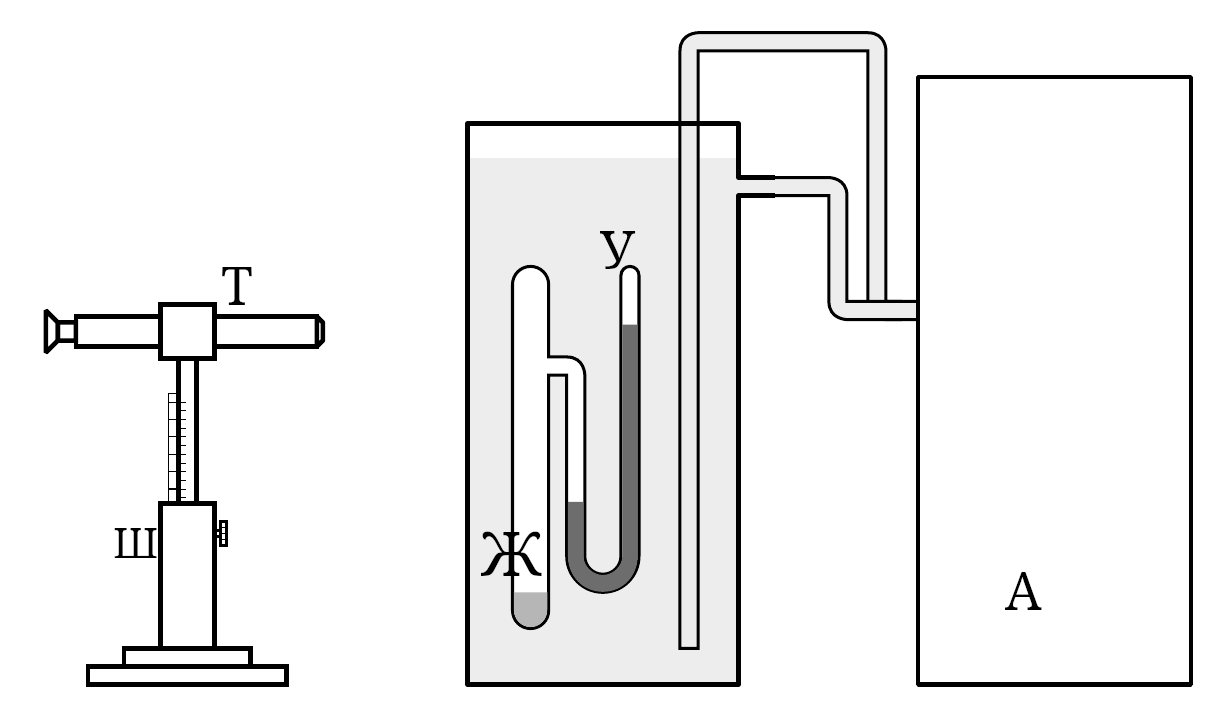
\includegraphics[scale = 0.19]{scheme.png}
  \caption{Экспериментальная установка.}
  \label{fig:img1}
\end{wrapfigure}
Экспериментальная установка изображена на рисунке~\ref{fig:img1}. Жидкости и ее пары находятся в ёмкости Ж. К ней-же для измерения давления подключена U-образная трубка У со ртутью в ней. Обе они герметичны и находятся в воде, температуру в которой поддерживает и измеряет термостат А. Для измерения высоты используется труба Т, закрепленная на штангенциркуле Ш. Совмещая отметку на стекле трубы со столбиками ртути путем изменения высоты трубки, можно измерить разность высот этих столбиков, тем самым определяя давление жидкости.
\subsection{Погрешности.}
\begin{itemize}
  \item Штангенциркуль: $\delta_{шт} = \pm 0,1 мм$.
  \item Термометр термостата: $\delta_{Т} = \pm 0,1\ ^{\circ}C$.
\end{itemize}
\section{Результаты измерений и обработка данных.}
\subsection{Результаты измерений.}
Проведем измерения температуры и давления. Для этого сначала постепенно нагревая воду до примерно 40 градусов, а потом остужая до комнатной температуры, будем измерять разность высот ртутных столбиков. Результаты измерений, а также рызница высот столбиков и давление пара, представлены в таблице~\ref{table:tab1}.
% Начало таблицы 1 {{{
\begin{table}[h!]
\centering
\begin{tabular}{ ||c|c|c|c|c|c|| }
  \hline
  №  & $T$, $К$  & $l_{ниж}$, см   & $l_{верх}$, см    & $\Delta l$, см  & $p$, Па \\
  \hline
  1  & $297,19 \pm 0,1$ & $6,60 \pm 0,01$ & $8,80 \pm 0,01$  & $2,20 \pm 0,02$ & $2930 \pm 3$ \\
  2  & $298,19 \pm 0,1$ & $6,55 \pm 0,01$ & $8,87 \pm 0,01$  & $2,32 \pm 0,02$ & $3090 \pm 3$ \\
  3  & $299,19 \pm 0,1$ & $6,48 \pm 0,01$ & $8,92 \pm 0,01$  & $2,44 \pm 0,02$ & $3250 \pm 3$ \\
  4  & $300,19 \pm 0,1$ & $6,34 \pm 0,01$ & $8,95 \pm 0,01$  & $2,61 \pm 0,02$ & $3476 \pm 3$ \\
  5  & $301,19 \pm 0,1$ & $6,24 \pm 0,01$ & $9,00 \pm 0,01$  & $2,76 \pm 0,02$ & $3676 \pm 3$ \\
  6  & $302,19 \pm 0,1$ & $6,14 \pm 0,01$ & $9,09 \pm 0,01$  & $2,95 \pm 0,02$ & $3929 \pm 3$ \\
  7  & $303,19 \pm 0,1$ & $6,08 \pm 0,01$ & $9,14 \pm 0,01$  & $3,06 \pm 0,02$ & $4075 \pm 3$ \\
  8  & $304,19 \pm 0,1$ & $6,00 \pm 0,01$ & $9,26 \pm 0,01$  & $3,26 \pm 0,02$ & $4342 \pm 3$ \\
  9  & $305,19 \pm 0,1$ & $5,93 \pm 0,01$ & $9,32 \pm 0,01$  & $3,39 \pm 0,02$ & $4515 \pm 3$ \\
  10 & $306,19 \pm 0,1$ & $5,83 \pm 0,01$ & $9,46 \pm 0,01$  & $3,63 \pm 0,02$ & $4835 \pm 3$ \\
  11 & $307,19 \pm 0,1$ & $5,73 \pm 0,01$ & $9,57 \pm 0,01$  & $3,84 \pm 0,02$ & $5114 \pm 3$ \\
  12 & $308,19 \pm 0,1$ & $5,70 \pm 0,01$ & $9,65 \pm 0,01$  & $3,95 \pm 0,02$ & $5261 \pm 3$ \\
  13 & $309,19 \pm 0,1$ & $5,50 \pm 0,01$ & $9,73 \pm 0,01$  & $4,23 \pm 0,02$ & $5634 \pm 3$ \\
  14 & $310,19 \pm 0,1$ & $5,39 \pm 0,01$ & $9,90 \pm 0,01$  & $4,51 \pm 0,02$ & $6007 \pm 3$ \\
  15 & $311,19 \pm 0,1$ & $5,25 \pm 0,01$ & $10,00 \pm 0,01$ & $4,75 \pm 0,02$ & $6327 \pm 3$ \\
  16 & $312,19 \pm 0,1$ & $5,13 \pm 0,01$ & $10,22 \pm 0,01$ & $5,09 \pm 0,02$ & $6779 \pm 3$ \\
  17 & $313,19 \pm 0,1$ & $5,00 \pm 0,01$ & $10,28 \pm 0,01$ & $5,28 \pm 0,02$ & $7032 \pm 3$ \\
  18 & $312,19 \pm 0,1$ & $5,15 \pm 0,01$ & $10,19 \pm 0,01$ & $5,04 \pm 0,02$ & $6713 \pm 3$ \\
  19 & $309,89 \pm 0,1$ & $5,39 \pm 0,01$ & $9,94 \pm 0,01$  & $4,55 \pm 0,02$ & $6060 \pm 3$ \\
  20 & $308,49 \pm 0,1$ & $5,58 \pm 0,01$ & $9,75 \pm 0,01$  & $4,17 \pm 0,02$ & $5554 \pm 3$ \\
  21 & $306,88 \pm 0,1$ & $5,72 \pm 0,01$ & $9,60 \pm 0,01$  & $3,88 \pm 0,02$ & $5168 \pm 3$ \\
  22 & $305,83 \pm 0,1$ & $5,83 \pm 0,01$ & $9,50 \pm 0,01$  & $3,67 \pm 0,02$ & $4888 \pm 3$ \\
  23 & $304,00 \pm 0,1$ & $6,03 \pm 0,01$ & $9,30 \pm 0,01$  & $3,27 \pm 0,02$ & $4362 \pm 3$ \\
  24 & $299,44 \pm 0,1$ & $6,20 \pm 0,01$ & $9,11 \pm 0,01$  & $2,91 \pm 0,02$ & $3876 \pm 3$ \\
  25 & $297,69 \pm 0,1$ & $6,58 \pm 0,01$ & $8,81 \pm 0,01$  & $2,23 \pm 0,02$ & $3023 \pm 3$ \\
  \hline
\end{tabular}
\caption{Результаты измерения разницы высот столбиков.}
\label{table:tab1}
\end{table}
% }}}
\newpage
\subsection{Обработка данных.}
\subsubsection{Графики.}
Построим график $P(T)$ на рисунке~2.
% Граф. 2 {{{
\begin{center}
\begin{tikzpicture}
\begin{axis}[
	xlabel = {$T$},
	ylabel = {$P$},
    grid = major,
	minor tick num = 6
]
\addplot[
    mark size=2pt,
    only marks,
    magenta,
]
table {
    x      y
    297.19 2930
    298.19 3090
    299.19 3250
    300.19 3476
    301.19 3676
    302.19 3929
    303.19 4075
    304.19 4342
    305.19 4515
    306.19 4835
    307.19 5114
    308.19 5261
    309.19 5634
    310.19 6007
    311.19 6327
    312.19 6779
    313.19 7032
};
\addplot[
    mark size=2pt,
    only marks,
    green,
]
table {
    x      y
    312.19 6713
    309.89 6060
    308.49 5554
    305.88 5168
    305.83 4888
    304.00 4362
    299.44 3476
    297.69 2970
};
\end{axis}
\end{tikzpicture}\newline
Рис. 2: График зависимости давления пара от его температуры.\newline
\end{center}
% }}}
Теперь погдотовим данные посроения графика с $1/T$ на оси абсцисс и $\ln P$ в качетсве ординат. На основании этих данных построим график (рис. 3).
% Начало таблицы 2 {{{
\begin{table}[h!]
\centering
\begin{tabular}{ ||c|c|c||c|c|c|| }
  \hline
  №  & $1/T \cdot 10^{-3}$ & $\ln P$ & №  & $1/T \cdot 10^{-3}$ & $\ln P$ \\
  \hline
  1  & $3,3365$ & $7,983$ &           14 & $3,3224$ & $8,701$ \\
  2  & $3,3354$ & $8,036$ &           15 & $3,3213$ & $8,753$ \\
  3  & $3,3342$ & $8,086$ &           16 & $3,3204$ & $8,822$ \\
  4  & $3,3331$ & $8,154$ &           17 & $3,3193$ & $8,858$ \\
  5  & $3,3332$ & $8,210$ &           18 & $3,3203$ & $8,811$ \\
  6  & $3,3309$ & $8,276$ &           19 & $3,3227$ & $8,706$ \\
  7  & $3,3298$ & $8,313$ &           20 & $3,3242$ & $8,622$ \\
  8  & $3,3287$ & $8,376$ &           21 & $3,3258$ & $8,550$ \\
  9  & $3,3277$ & $8,415$ &           22 & $3,3268$ & $8,494$ \\
  10 & $3,3265$ & $8,484$ &           23 & $3,3289$ & $8,381$ \\
  11 & $3,3255$ & $8,540$ &           24 & $3,3313$ & $8,263$ \\
  12 & $3,3245$ & $8,568$ &           25 & $3,3359$ & $7,996$ \\
  13 & $3,3234$ & $8,637$ & & & \\

  \hline
\end{tabular}
\caption{Результаты измерения разницы высот столбиков.}
\label{table:tab2}
\end{table}
% }}}
% Граф. 3 {{{
\begin{center}
\begin{tikzpicture}
\begin{axis}[
	xlabel = {$1/T \cdot 10^{-3}$},
	ylabel = {$\ln P$},
  xmin = 3.317,
  xmax = 3.34,
  ymin = 7.8,
  ymax = 8.983,
  grid = major,
	minor tick num = 6
]
\addplot[
    mark size=2pt,
    only marks,
    blue,
]
table {
    x     y
    3.3365 7.983
    3.3354 8.036
    3.3342 8.086
    3.3331 8.154
    3.3332 8.210
    3.3309 8.276
    3.3298 8.313
    3.3287 8.376
    3.3277 8.415
    3.3265 8.484
    3.3255 8.540
    3.3245 8.568
    3.3234 8.637
    3.3224 8.701
    3.3213 8.753
    3.3204 8.822
    3.3193 8.858
};
\addplot[
    mark size=2pt,
    only marks,
    red,
]
table {
    x      y
    3.3203 8.811
    3.3227 8.706
    3.3242 8.622
    3.3258 8.550
    3.3268 8.494
    3.3289 8.381
    3.3313 8.263
    3.3359 7.996
};
\addplot[
    no marks,
    % yes, Marx
    black,
]
table {
    x     y
    3.317 8.980
    3.34  7.8
    % 3.317 8.2270816
    % 3.34  8.1090218
};
\end{axis}
\end{tikzpicture}\newline
Рис. 3: График зависимости $\ln P$ от $1/T$.\newline
\end{center}
% }}}
Как видно, второй график куда лучше подходит для вычислений, так как и в теории, и на практике представляет из себя прямую, что позволяет найти искомую производную путем аппроксимации. Аппроксимируем график к прямой и найдем угловой коэффицент:\newline
$b = \frac{ \left< xy \right> - \left< x \right> \left< y \right> }{ \left< x^{2} \right> - \left< x \right>^{2} } = -5130 \pm 100$.\newline
$L_{моль} = b \cdot R = 4267 \pm 83\ \frac{Дж}{моль}$.\newline
$L_{кг} = L_{моль} / \mu_{в} = 237000 \pm 4600 \ \frac{Дж}{г}$.
\section{Выводы.}
В ходе работы косвенным методом была вычислена удельная теплота парообразования воды. Табличное значение находится в пределах погрешности, а сама относительная погрешность составляет $2\%$, что позволяет считать расчеты достаточно точными.
\end{document}
